\documentclass[
  12pt,
  a4paper,
  twoside,
  openright,
]{memoir}

\usepackage{float}
\usepackage{calc}
\usepackage{tasks}
\usepackage{lipsum}
\usepackage{fontspec}                    % Load and configure
% OpenType/TrueType fonts (LuaLaTeX/XeLaTeX)
\usepackage{amsmath}
\usepackage{amsthm}
\usepackage{amssymb}                     % Additional mathematical symbols
\usepackage{mathtools}                   % Enhanced mathematical
% typesetting (loads amsmath)
\usepackage{unicode-math}                % Unicode and OpenType math fonts
\usepackage{microtype}                   % Improved typography and %
% character protrusion
\usepackage{tikz}                        % Create vector graphics and diagrams
\usepackage{graphicx}                    % Include and manipulate images
\usepackage{witharrows}                  % Annotating with arrows inside Latex
\usepackage{adjustbox}
\usepackage{empheq}
\usepackage{pifont}
\usepackage{booktabs}                    % Professional-quality tables
\usepackage{array}                       % Extended table column formatting
\usepackage{enumitem}                    % Customize lists and enumerations
\usepackage{csquotes}                    % Context-sensitive quotation marks
\usepackage[most]{tcolorbox}             % Colored and framed boxes
\usepackage{etoolbox}                    % A toolbox of programming facilities
\usepackage{etoc}
\usepackage{caption}
\usepackage[dvipsnames,svgnames]{xcolor} % Extended color support
\usepackage{cancel}                      % Draw cancellation marks in math
\usepackage{siunitx}                     % Typeset numbers and SI units
\usepackage{nicematrix}                  % Enhanced matrices and arrays
\usepackage[normalem]{ulem}              % Underline with more robust linebreak
% \usepackage{tikz-cd}                   % Commutative diagrams with TikZ
\usepackage{multicol}                    % Create multicolumn lists
\usepackage{hyperref}                    % Hyperlinks, PDF metadata,
% and cross-references
\usepackage{bookmark}                    % Faster and more robust PDF bookmarks

\defaultfontfeatures{
  Ligatures=TeX,
  Scale=1.2,
}
\setlength{\parindent}{0pt}
\nonzeroparskip
\linespread{1.4}
\newfontfamily\emojifont{Noto Emoji}
\newfontfamily\coloremojifont{Noto Color Emoji}
\newfontfamily\notosanssymbols{Noto Sans Symbols 2}
%\setmainfont{Libertinus Sans}
%\setsansfont{Libertinus Sans}
%\setmonofont{Libertinus Mono}
%\setmathfont{Libertinus Math}
\setmainfont{Noto Sans}
\setsansfont{Noto Sans}
\setmonofont{Noto Sans Mono}
\setmathfont[
Path=fonts/,
Extension=.ttf
]{NotoSansMath-Regular}

\hypersetup{
  colorlinks=true,
  linkcolor=black,
  urlcolor=blue,
  citecolor=black,
  bookmarksdepth=3,
  bookmarksnumbered=true,
  bookmarksopen=true
}
\setstocksize{297mm}{210mm}
\settrimmedsize{\stockheight}{\stockwidth}{*}
% \settypeblocksize{220mm}{130mm}{*}
\setlrmarginsandblock{12mm}{12mm}{*}
\setulmarginsandblock{20mm}{15mm}{*}
\checkandfixthelayout
\setsecnumdepth{section}

\makechapterstyle{mystyle}{%
  % Chapter
  \renewcommand{\chapnamefont}{\Huge\bfseries\color{MidnightBlue}}
  \renewcommand{\chapnumfont}{\Huge\bfseries\color{MidnightBlue}}
  \renewcommand{\chaptitlefont}{\Huge\bfseries\color{MidnightBlue}}

  % Section
  \setsecheadstyle{%
    \Large\bfseries\color{MidnightBlue}
  }

  % Subsection
  \setsubsecheadstyle{%
    \large\bfseries\color{MidnightBlue}
    \MakeUppercase
  }

  % Subsubsection
  \setsubsubsecheadstyle{%
    \normalsize\bfseries\color{MidnightBlue}
  }
}

\chapterstyle{mystyle}

% Line spacing
\linespread{1.4}

% Paragraph spacing
\setlength{\parindent}{0pt}
\nonzeroparskip

% Display math spacing
\setlength{\abovedisplayskip}{1pt}
\setlength{\belowdisplayskip}{1pt}

\captionsetup{
  font=small
}

\setlist[itemize]{
  label=\textbullet,
  leftmargin=*,
  % itemsep=0.5em,
  % topsep=0.5em,
  % nosep,
}

\setlist[enumerate]{
  label=(\alph*),
  leftmargin=2em,
  topsep=0pt,
  partopsep=0pt,
  itemsep=\parskip,
  parsep=0pt,
}

\newcommand{\headerfont}{%
  \footnotesize\sffamily
}
\makepagestyle{textbook}
\makeheadrule{textbook}{\textwidth}{0pt}
\makeevenfoot{textbook}{}{}{}
\makeoddfoot{textbook}{}{}{}

\makeevenhead{textbook}
{\headerfont\leftmark}
{}
{\headerfont\thepage}


\makeoddhead{textbook}
{\headerfont\rightmark}
{}
{\headerfont\thepage}

\pagestyle{textbook}
\makepagestyle{chapterstyle}
\makeevenhead{chapterstyle}{}{}{}
\makeoddhead{chapterstyle}{}{}{}
\makeheadrule{chapterstyle}{\textwidth}{0pt}
\makeevenfoot{chapterstyle}{}{\headerfont\thepage}{}
\makeoddfoot{chapterstyle}{}{\headerfont\thepage}{}
\aliaspagestyle{chapter}{chapterstyle}
\aliaspagestyle{plain}{chapterstyle}
\tcbuselibrary{theorems,skins}

\tcbset{
  textbookbox/.style={
    breakable,
    %    parbox=false,
    enhanced,
    boxrule=1pt,
    arc=2mm,
    fonttitle=\normalsize\bfseries,
    left=0.5em,
    right=0.5em,
    top=1.5em,
    bottom=0.5em,
    before skip=1em,
    after skip=1em,
    colback=white,
    colframe=black,
    coltitle=black,
    before upper app={\nonzeroparskip},
    attach boxed title to top left={
      xshift=4mm,
      yshift=-\tcboxedtitleheight/2
    },
    boxed title style={
      colback=white,
      colframe=black,
      boxrule=1pt,
    }
  }
}
\newcounter{postulate}[section]
\renewcommand{\thepostulate}{\arabic{postulate}}

\newenvironment{postulate}
{%
  \refstepcounter{postulate}%
  \begin{tcolorbox}[
    textbookbox,
    title=\textbf{Postulate \thepostulate},
    colback=teal!5,
    colframe=teal,
    coltitle=white,
    boxed title style={
      colback=teal,
      colframe=teal,
      boxrule=1pt,
      top=2pt,
      bottom=2pt,
      left=4pt,
      right=4pt,
    }
    ]
  }
  {
\end{tcolorbox}}

\newcounter{example}[section]
\renewcommand{\theexample}{\arabic{example}}

\newenvironment{example}
{%
  \refstepcounter{example}%
  \begin{tcolorbox}[
    textbookbox,
    title=\textbf{Example \theexample},
    colback=violet!5,
    colframe=violet,
    coltitle=white,
    boxed title style={
      colback=violet,
      colframe=violet,
      boxrule=1pt,
      top=4pt,
      bottom=2pt,
      left=4pt,
      right=4pt,
    }
    ]
  }
  {
  \end{tcolorbox}
}

\newenvironment{solution}
{\par\noindent\textbf{Solution}\ignorespaces}
{\par}


\begin{document}

\frontmatter

\begin{titlingpage}

	\centering

	\vspace*{\fill}

	{\Huge Geometry}\\[2em]

	{\Large A Modern Introduction}

	\vspace*{\fill}

	Roman Steinberger

\end{titlingpage}


\tableofcontents

\etocsettocstyle{}{}

\chapter{Preface}

Geometry is the study of the properties and relationships of figures in the plane and in space. Since the time of Euclid, it has served as one of the principal means by which students learn the nature of logical reasoning and mathematical proof. From a small collection of definitions, postulates, and previously established results, an extensive body of knowledge is developed through careful deduction.

The purpose of this book is to present the fundamental principles of Euclidean geometry in a clear, orderly, and systematic manner. Each topic is introduced with precise definitions and illustrated by examples and diagrams before being reinforced through exercises of varying difficulty. Throughout the text, emphasis is placed not only on obtaining correct answers but also on understanding the reasoning that justifies them.

Geometry is more than the study of shapes and measurements. It provides a framework for analyzing patterns, making logical arguments, and solving problems with precision. These skills are of lasting value in mathematics, the sciences, engineering, architecture, and many other disciplines.

The reader is encouraged to approach each new topic thoughtfully, to examine every diagram carefully, and to develop the habit of proving statements rather than accepting them by intuition alone. Mastery of geometry is achieved through patient study, regular practice, and an appreciation for the logical structure that unifies the subject.

It is hoped that this book will provide a firm foundation in geometry and foster an enduring appreciation for the elegance, rigor, and usefulness of mathematical reasoning.


\mainmatter

\chapter{Essentials of Geometry}

\localtableofcontents*

\textbf{Perimeter}: The distance around a rectangle is called its
\textbf{perimeter.}

\textbf{Circumference}: The distance around a circle is called its
\textbf{circumference.}

% \settasks{
%   label-width=0em,
%   label=\makebox[0pt][r]{\textbf{\arabic*.}},
%   item-indent=2em,
% }

% \begin{tasks}(4) % 3 columns
%   \task one
%   \task one
%   \task one
%   \task one
%   \task one
%   \task one
%   \task one
%   \task one
% \end{tasks}

\section{Points, Lines, and Planes}

\subsection{Undefined Terms}

In geometry, the words \textit{point}, \textit{line},
and \textit{plane} are undefined terms.
These words do not have formal definitions, but there is agreement about
what they mean.

\textcolor{blue}{\textbf{Point}} A point has no dimension. It is
represented by a dot.

{
  \par\centering
  
\includegraphics[width=0.06\textwidth]{figures/1/1-1.pdf}\\
  {\small point \(A\)}
  \par
}

\textcolor{blue}{\textbf{Line}} A line has one dimension. It is
represented by a line with two arrowheads,
but it extends without end.

Through any two points, there is exactly one
line. You can use any two points on a line
to name it.

{
  \par\centering
  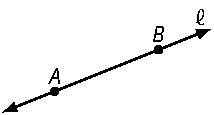
\includegraphics[width=0.3\textwidth]{figures/1/1-2.pdf}\\
  {\small line \(\ell\), line \(AB\) (\(\overleftrightarrow{AB}\)),
  or line \(BA\) (\(\overleftrightarrow{BA}\))}
  \par
}

\textcolor{blue}{\textbf{Plane}} A plane has two dimensions. It is
represented by a shape that looks like a floor
or a wall, but it extends without end.

Through any three points not on the same line, there is exactly one
plane. You can use three points that are not all on the same line to
name a plane.

{
  \par\centering
  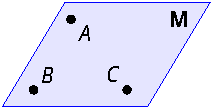
\includegraphics[width=0.3\textwidth]{figures/1/1-3.pdf}\\
  {\small plane \(\symbf{M}\) or plane \(ABC\)}
  \par
}

\textcolor{blue}{\textbf{Collinear points}} Collinear points are
points that lie on
the same line.

\textcolor{blue}{\textbf{Coplanar points}} Coplanar points are points
that lie in the same plane.

\begin{example}\label{exa:point}

  \textcolor{violet}{\textbf{Name points, lines, and planes}}

  {
    \par\centering
    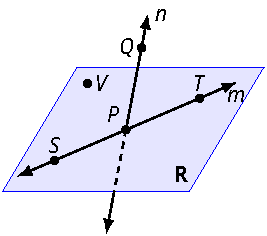
\includegraphics[width=0.35\textwidth]{figures/1/1-4.pdf}
    \par
  }

  \begin{enumerate}[]
    \item Give two other names for \(\overleftrightarrow{PQ}\)

    \item Give two other names for plane \(\symbf{R}\).

    \item Name three points that are collinear.

    \item Name four points that are coplanar.

  \end{enumerate}

  \begin{solution}
    \begin{enumerate}
      \item Line \(n\), \(\overleftrightarrow{QP}\).

      \item Plane \(VST\), plane \(VPT\).

      \item Points \(S\), \(P\), and \(T\).

      \item Points \(V\), \(S\), \(P\), and \(T\).

    \end{enumerate}
  \end{solution}
\end{example}

\subsection{Defined Terms}

In geometry, terms that can be described using known
words such as \textit{point} or \textit{line} are called defined terms.

Line \(AB\) (written as \(\overleftrightarrow{AB}\)) and points \(A\)
and \(B\) are
used here to define the terms below.

{
  \par\centering
  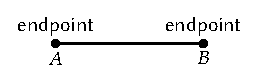
\includegraphics[width=0.3\textwidth]{figures/1/1-5.pdf}\\
  {\small line \(\overleftrightarrow{AB}\)}
  \par
}

\textcolor{blue}{\textbf{Segment}} The line segment \(AB\), or segment \(AB\),
(written as \(\overline{AB}\)) consists of the endpoints \(A\) and
\(B\) and all points on \(\overleftrightarrow{AB}\)
that are between \(A\) and \(B\).

Note that \(\overline{AB}\) can also be named \(\overline{BA}\).

{
  \par\centering
  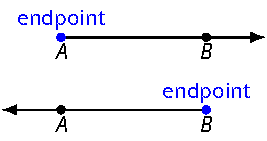
\includegraphics[width=0.3\textwidth]{figures/1/1-6.pdf}\\
  {\small segment \(\overline{AB}\) or \(\overline{BA}\)}
  \par
}

\textcolor{blue}{\textbf{Ray}} The ray \(AB\) (written as
\(\overrightarrow{AB}\)) consists of
the point \(A\) and all points on \(\overleftrightarrow{AB}\) that lie on the
same side of \(A\) as \(B\).

Note that \(\overrightarrow{AB}\) and \(\overrightarrow{BA}\) are
different rays.

{
  \par\centering
  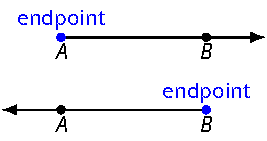
\includegraphics[width=0.35\textwidth]{figures/1/1-7.pdf}\\
  {\small rays $\overrightarrow{AB}$ and $\overrightarrow{BA}$}
  \par
}

\textcolor{blue}{\textbf{Opposite rays}} If point \(C\) lies on
\(\overleftrightarrow{AB}\) between
\(A\) and \(B\), then \(\overrightarrow{CA}\) and \(\overrightarrow{CB}\)
are opposite rays.

{
  \par\centering
  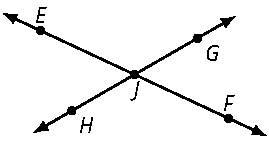
\includegraphics[width=0.35\textwidth]{figures/1/1-8.pdf}\\
  {\small opposite rays \(\overrightarrow{CA}\) and \(\overrightarrow{CB}\)}
  \par
}

Segments and rays are collinear if they lie on the same line. So, opposite rays
are collinear. Lines, segments, and rays are coplanar if they lie in the
same plane.

\begin{example}
  \textcolor{violet}{\textbf{Name segments, rays, and opposite rays}}

  {
    \par\centering
    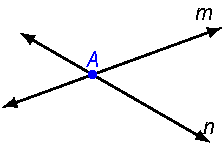
\includegraphics[width=0.35\textwidth]{figures/1/1-9.pdf}
    \par
  }

  \begin{enumerate}
    \item Give another name for \(\overline{GH}\).

    \item Name all rays with endpoint \(J\). Which of these rays are
      opposite rays?

  \end{enumerate}

  \begin{solution}
    \begin{enumerate}
      \item Another name for \(\overrightarrow{GH}\) is \(\overrightarrow{HG}\).

      \item The rays with endpoint \(J\) are \(\overrightarrow{JE}\),
        \(\overrightarrow{JG}\), \(\overrightarrow{JF}\), and
        \(\overrightarrow{JH}\).

        The pairs of opposite rays with endpoint \(J\) are
        \(\overrightarrow{JE}\)
        and \(\overrightarrow{JF}\), and \(\overrightarrow{JG}\) and
        \(\overrightarrow{JH}\).

    \end{enumerate}
  \end{solution}
\end{example}

\subsection{Intersections}

\textcolor{blue}{\textbf{Intersection}} Two or more geometric
figures intersect if
they have one or more points in common. The intersection of the
figures is the set of points
the figures have in common. Some examples of intersections are shown below.

{
  \par\centering
  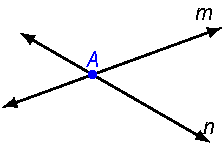
\includegraphics[width=0.3\textwidth]{figures/1/1-10.pdf}\\
  {\small The intersection of two different lines is a point.}
  \par
}

{
  \par\centering
  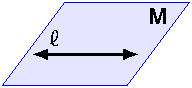
\includegraphics[width=0.3\textwidth]{figures/1/1-11.pdf}\\
  {\small The intersection of two different planes is a line.}
  \par
}

\begin{example}
  \textcolor{violet}{\textbf{Sketch intersections of lines and planes}}

  \begin{enumerate}
    \item Sketch a plane and a line that is in the plane.

    \item Sketch a plane and a line that does not intersect the plane.

    \item Sketch a plane and a line that intersects the plane at a point.
  \end{enumerate}
  \begin{solution}
    \begin{enumerate}
      \item The line \(\ell\) is in the plane \(\symbf{M}\).

        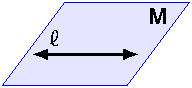
\includegraphics[width=0.3\textwidth]{figures/1/1-12.pdf}

      \item The line \(\ell\) does not intersect the plane \(\symbf{M}\).

        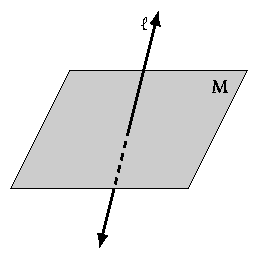
\includegraphics[width=0.3\textwidth]{figures/1/1-13.pdf}

      \item The line \(\ell\) intersects the plane \(\symbf{M}\) at a point.

        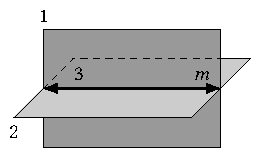
\includegraphics[width=0.3\textwidth]{figures/1/1-14.pdf}
    \end{enumerate}
  \end{solution}
\end{example}

\begin{example}
  \textcolor{violet}{\textbf{Sketch intersections of planes}}

  Sketch two planes that intersect in a line.

  \begin{solution}

    step 1 Draw a vertical plane. Shade the plane.

    step 2 Draw a second plane that is
    horizontal. Shade this plane a
    different color. Use dashed lines to
    show where one plane is hidden.

    step 3 Draw the line of intersection.

    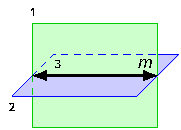
\includegraphics[width=0.35\textwidth]{figures/1/1-15.pdf}

  \end{solution}
\end{example}

\section{Use Segments and Congruence}

\textcolor{blue}{Postulate} In Geometry, a rule that is accepted without
proof is called a postulate or axiom.

\textcolor{blue}{Theorem} A rule that can be proved is called a theorem.

\begin{postulate}

  \textcolor{teal}{\textbf{Ruler Postulate}}

  The points on a line can be matched one
  to one with the real numbers. The real
  number that corresponds to a point is the
  \textbf{coordinate} of the point.

  {
    \par\centering
    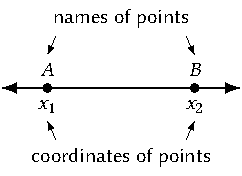
\includegraphics[width=0.4\textwidth]{figures/1/2-1.pdf}
    \par
  }

  The \textbf{distance} between points \(A\) and \(B\),
  written as \(AB\), is the absolute value of the
  difference of the coordinates of \(A\) and \(B\).

  {
    \par\centering
    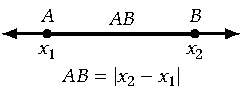
\includegraphics[width=0.4\textwidth]{figures/1/2-2.pdf}
    \par
  }
\end{postulate}

The distance between points \(A\) and \(B\), or \(AB\),
is also called the \textit{length} of \(\overline{AB}\).

\subsection{Adding Segment Lengths}

When three points are collinear, you can say
that one point is \textbf{between} the other two.
%\makebox[\textwidth][c]{%
%  \begin{minipage}[t]{0.35\textwidth}
%    \centering
%    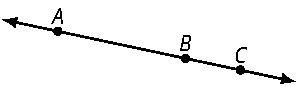
\includegraphics[width=\linewidth]{figures/1/2-3.pdf}
%
%    {\small Point \(B\) is between points \(A\) and \(C\).}
%  \end{minipage}\hspace{0.05\textwidth}
%  \begin{minipage}[t]{0.35\textwidth}
%    \centering
%    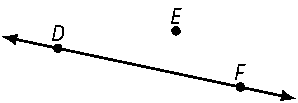
\includegraphics[width=\linewidth]{figures/1/2-4.pdf}
%
%    {\small Point \(E\) is not between points \(D\) and \(F\).}
%  \end{minipage}
%}
{
  \par\centering
  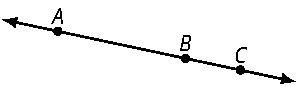
\includegraphics[width=0.4\textwidth]{figures/1/2-3.pdf}\\
  {\small Point \(B\) is between points \(A\) and \(C\).}
  \par
}
{
  \par\centering
  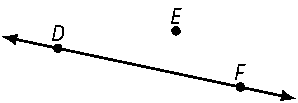
\includegraphics[width=0.4\textwidth]{figures/1/2-4.pdf}\\
  {\small Point \(E\) is not between points \(D\) and \(F\).}
  \par
}

\begin{postulate}
  \textcolor{teal}{\textbf{Segment Addition Postulate}}

  If \(B\) is between \(A\) and \(C\), then \(AB+BC=AC\).
  If \(AB+BC=AC\), then \(B\) is between \(A\) and \(C\).

  {
    \par\centering
    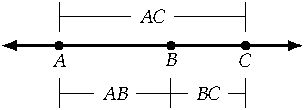
\includegraphics[width=0.35\textwidth]{figures/1/2-5.pdf}
    \par
  }
\end{postulate}

\begin{example}
  \textcolor{violet}{\textbf{Find a length}}

  Use the diagram to find \(GH\).

  {
    \par\centering
    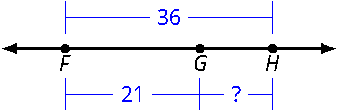
\includegraphics[width=0.35\textwidth]{figures/1/2-6.pdf}\\
  }
  \begin{solution}

    Use the Segment Addition Postulate to write an equation. Then solve the
    equation to find \(GH\).
    \[
      \begin{aligned}
        FH &= FG+GH && \text{Segment Addition Postulate}\\
        36 &= 21+GH && \text{Substitute $36$ for $FH$ and $21$ for $FG$.}\\
        15 &= GH    && \text{Subtract $21$ from each side.}
      \end{aligned}
    \]
  \end{solution}
\end{example}

\subsection{Congruent Segments}

Line segments that have the same length are called
\textbf{congruent segments}. In the diagram below, you can say “the length of
\(\overline{AB}\) is equal to the length of \(\overline{CD}\),”
or you can say “\(\overline{AB}\) is congruent to \(\overline{CD}\).”
The symbol \(\cong\) means “is congruent to.”

\makebox[\textwidth][c]{%
  \begin{minipage}[t]{0.22\textwidth}
    \centering
    \adjustbox{valign=t}{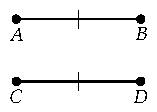
\includegraphics[width=\linewidth]{figures/1/2-7.pdf}}
  \end{minipage}\hspace{0.01\textwidth}
  \begin{minipage}[t]{0.35\textwidth}
    \centering
    Lengths are equal.\\
    \(AB=CD\)\\
    \(\uparrow\)\\
    "is equal to"
  \end{minipage}\hspace{0.01\textwidth}
  \begin{minipage}[t]{0.35\textwidth}
    \centering
    Segments are congruent.\\
    \(\overline{AB}\cong\overline{CD}\)\\
    \(\uparrow\)\\
    "is congruent to"
  \end{minipage}
}

\begin{example}
  \textcolor{violet}{\textbf{Compare segments for congruence}}

  Plot \(J(23, 4)\), \(K(2, 4)\), \(L(1, 3)\), and \(M(1, 22)\) in a
  coordinate plane.
  Then determine whether \(\overline{JK}\) and \(\overline{LM}\) are congruent.

  \begin{solution}
    %    \makebox[\textwidth][c]{%
    %      \begin{minipage}[t]{0.56\textwidth}
    %        To find the length of a horizontal segment,
    %        find the absolute value of the difference of
    %        the \(x\)-coordinates of the endpoints.
    %        \[
    %        JK=|2-(-3)|=5 \quad \text{Use Ruler Postulate.}
    %        \]
    %        To find the length of a vertical segment,
    %        find the absolute value of the difference of
    %        the \(y\)-coordinates of the endpoints.
    %        \[
    %        LM=|-2-3|=5 \quad \text{Use Ruler Postulate.}
    %        \]
    %        \(JK\) and \(LM\) have the same length. So,
    %        \(\overline{JK}\cong\overline{LM}\).
    %      \end{minipage}\hspace{0.02\textwidth}
    %      \begin{minipage}[t]{0.36\textwidth}
    %        \centering
    %        \adjustbox{valign=t}{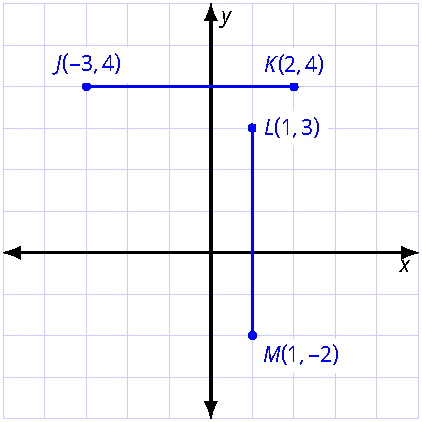
\includegraphics[width=\linewidth]{figures/1/2-8.pdf}}
    %      \end{minipage}
    %    }
    {
      \par\centering
      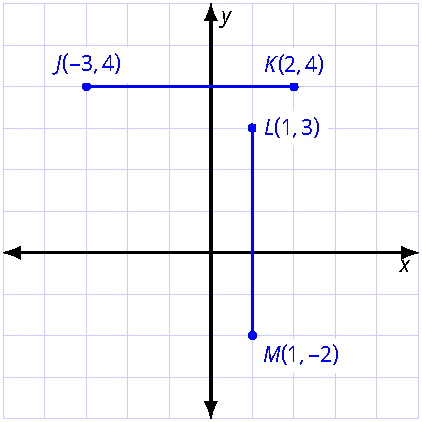
\includegraphics[width=0.4\textwidth]{figures/1/2-8.pdf}
      \par
    }

    To find the length of a horizontal segment,
    find the absolute value of the difference of
    the \(x\)-coordinates of the endpoints.
    \[
      JK=|2-(-3)|=5 \quad \text{Use Ruler Postulate.}
    \]
    To find the length of a vertical segment,
    find the absolute value of the difference of
    the \(y\)-coordinates of the endpoints.
    \[
      LM=|-2-3|=5 \quad \text{Use Ruler Postulate.}
    \]
    \(JK\) and \(LM\) have the same length. So,
    \(\overline{JK}\cong\overline{LM}\).

  \end{solution}
\end{example}

\section{Use Midpoint and Distance Formulas}

\subsection{Midpoints and Bisectors}

The \textbf{midpoint} of a segment is the point that
divides the segment into two congruent segments. A \textbf{segment bisector} is
a point, ray, line, line segment, or plane th at intersects the segment at its
midpoint. A midpoint or a segment bisector \textit{bisects} a segment.

%\makebox[\textwidth][c]{%
%\begin{minipage}[t]{0.45\textwidth}
%  \centering
%  \adjustbox{valign=t}{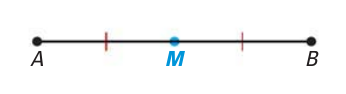
\includegraphics[width=\linewidth]{figures/1/3-1.png}}
%  {\small \(M\) is the midpoint of \(\overline{AB}\).
%    So \(\overline{AM}\cong\overline{MB}\) and \(AM=MB\)}
%\end{minipage}\hspace{0.02\textwidth}
%\begin{minipage}[t]{0.45\textwidth}
%  \centering
%  \adjustbox{valign=t}{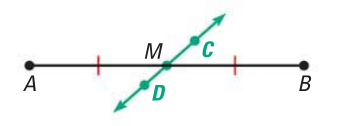
\includegraphics[width=\linewidth]{figures/1/3-2.png}}
%  {\small \(CD\) is a segment bisector of \(AB\).
%  So, \(\overline{AM}\cong\overline{MB}\) and \(AM=MB\).}
%\end{minipage}
%}
{
  \par\centering
  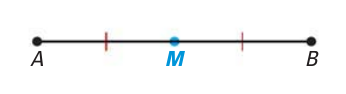
\includegraphics[width=0.4\textwidth]{figures/1/3-1.png}\\
  {\small \(M\) is the midpoint of \(\overline{AB}\).
  So \(\overline{AM}\cong\overline{MB}\) and \(AM=MB\).}
  \par
}
{
  \par\centering
  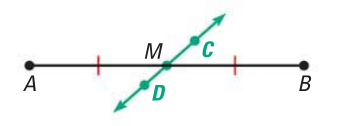
\includegraphics[width=0.4\textwidth]{figures/1/3-2.png}\\
  {\small \(CD\) is a segment bisector of \(AB\).
  So, \(\overline{AM}\cong\overline{MB}\) and \(AM=MB\).}
  \par
}

\begin{example}
  \textcolor{violet}{\textbf{Find segment lengths}}

  In the skateboard design, \(VW\) bisects \(XY\) at
  point \(T\), and \(XT=\qty{39.9}{\centi\meter}\). Find \(XY\).

  {
    \par\centering
    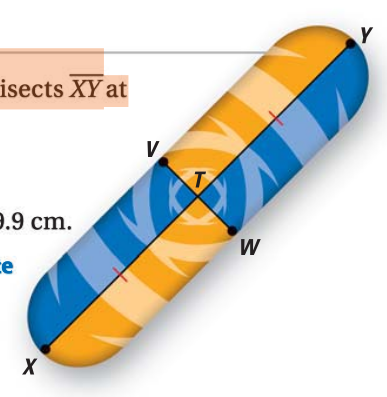
\includegraphics[width=0.3\textwidth]{figures/1/3-3.png}
    \par
  }

  \begin{solution}
    Point \(T\) is the midpoint of \(XY\). So,
    \(XT=TY=\qty{39.9}{\centi\meter}\).
    \[
      \begin{aligned}
        XY &= XT+TY & \quad \text{Segment Addition Postulate}\\
        &= 39.9+39.9\\
        &=79.8\unit{\centi\meter}
      \end{aligned}
    \]
  \end{solution}

\end{example}

\begin{example}
  \textcolor{violet}{Use algebra with segment lengths}

  Point \(M\) is the midpoint of \(\overline{VW}\).
  Find the length of \(\overline{VM}\).

  {
    \par\centering
    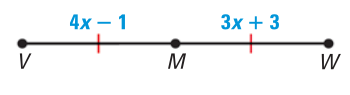
\includegraphics[width=0.3\textwidth]{figures/1/3-4.png}
    \par
  }

  \begin{solution}

    step~1 Write and solve an equation. Use the fact that that \(VM=MW\).
    \[
      \begin{aligned}
        VM &= MW          && \quad \text{Write equation.}\\
        4x - 1 &= 3x - 3  && \quad \text{Substitute.}\\
        x-1 &= 3          && \quad \text{Subtract \ensuremath{3x}
        from each side.}\\
        x &= 4            && \quad \text{Add 1 to each side.}
      \end{aligned}
    \]
    step~2 Evaluate the expression for \(VM\) when \(x = 4\).
    \[VM=4x-1=4(4)-1=15\]
    So the length of \(\overline{VM}\) is \boxed{15}.

    check Because \(VM = MW\), the length of \(\overline{MW}\)
    should be \(15\). If you evaluate the expression for \(MW\),
    you should find that \(MW = 15\).
    \[MW=3x+3=3(4)+3=15 \checkmark\]
  \end{solution}
\end{example}

You can use the coordinates of the endpoints of a
segment to find the coordinates of the midpoint.

\subsection{The Midpoint Formula}

The coordinates of the midpoint of a
segment are the averages of the
\(x\)-coordinates and of the \(y\)-coordinates
of the endpoints.

If \(A(x_1, y_1)\) and \(B(x_2, y_2)\) are points in a
coordinate plane, then the midpoint \(M\)
\(\overline{AB}\) has coordinates
\[
  \left( \frac{x_1+x_2}{2}, \frac{y_1+y_2}{2} \right)
\]
{
  \par\centering
  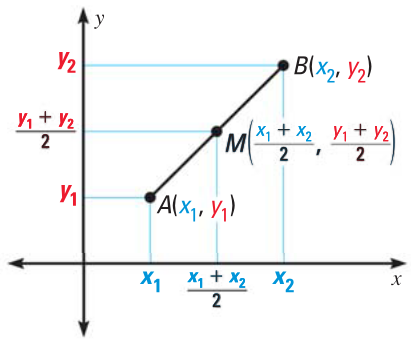
\includegraphics[width=0.4\textwidth]{figures/1/3-5.png}
  \par
}

\begin{example}

  \textcolor{violet}{\textbf{Use the Midpoint Formula}}
  \begin{enumerate}

    \item The endpoints of \(\overline{RS}\) are \(R(1, -3)\) and
      \(S(4, 2)\). Find
      the coordinates of the midpoint \(M\).

      {
        \par\centering
        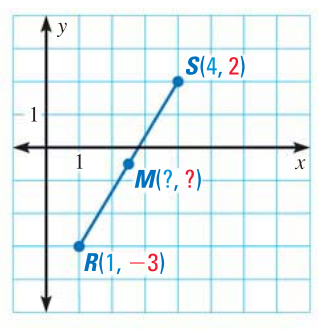
\includegraphics[width=0.35\textwidth]{figures/1/3-6.png}
        \par
      }

    \item The midpoint of \(\overline{JK}\) is \(M(2, 1)\). One endpoint is
      \(J(1, 4)\). Find the coordinates of endpoint \(K\).

      {
        \par\centering
        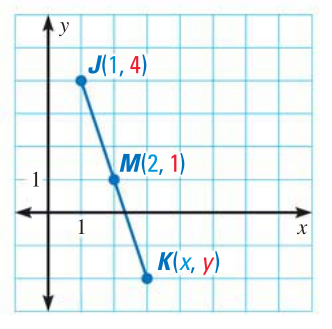
\includegraphics[width=0.35\textwidth]{figures/1/3-7.png}
        \par
      }
  \end{enumerate}
  \begin{solution}

    \begin{enumerate}
      \item Use the Midpoint Formula.
        \[
          M\left(\frac{1+4}{2},\frac{-3+2}{2}\right)=
          M\left(\frac{5}{2},-\frac{1}{2}\right)
        \]
        The coordinates of the midpoint M are
        \boxed{\left(\frac{5}{2},-\frac{1}{2}\right)}.

      \item Let \((x, y)\) be the coordinates of endpoint \(K\).
        Use the Midpoint Formula.

        step~1 Find \(x\).
        \[
          \begin{aligned}
            \frac{1+x}{2} &= 2\\
            1+x &= 4\\
            x &= 3
          \end{aligned}
        \]
        step~2 Find \(y\).
        \[
          \begin{aligned}
            \frac{4+y}{2} &= 1\\
            4+y &= 2\\
            y &= -2
          \end{aligned}
        \]
        The coordinates of endpoint \(K\) are \boxed{(3, -2)}.
    \end{enumerate}
  \end{solution}
\end{example}

\subsection{DISTANCE FORMULA}

The Distance Formula is a formula for computing the
distance between two points in a coordinate plane.

%%%%%%%%%%%%%%%%%%%%%%%%%%%%%%%%%%%%%%%%%%%%%%%%%%%%%%%%%%%%
% Back Matter
%%%%%%%%%%%%%%%%%%%%%%%%%%%%%%%%%%%%%%%%%%%%%%%%%%%%%%%%%%%%

\backmatter

\chapter{Appendix}

\lipsum[21-22]

\end{document}
